\chapter{Higgs Combination and Properties}
\label{chap:combinations}

%Careful not to get phillosphical, this section is about
%combined searches not really about stats.
\emph{The sensitivity 
of the search for the SM Higgs boson depends not only on the production cross-section and 
branching ratio to a particular decay channel, but also on the efficiency
of the selection, the experimental resolution and the relative proportions of 
signal to background processes. These quantities typically vary greatly as a function of 
$\mh$. By combining results from searches
in many decay channels, over a large range in mass, 
the overall sensitivity is greatly improved.
This chapter describes the combined searches for the SM Higgs and measurements of its properties. 
In Section~\ref{sec:combinationmethodology}, a short review on the statistical 
treatment of data from different analyses used at CMS is provided and a set of diagnostic
tools developed by the author are discussed.
The results of the search using the 2012 International Conference on
High Energy Physics (ICHEP 2012) dataset, 
which led to the announcement of the discovery of a new particle 
by ATLAS and CMS in July 2012~\citep{HIG-12-028}, are included.
Section~\ref{sec:properties} deals with early studies of the 
properties of the newly discovered particle presented at the Hadron Collider Physics (HCP) 
symposium in November 2012. This includes a discussion of 
the Feldman-Cousins technique which was implemented and performed
by the author to extract information on the compatibility of the new 
state with the SM Higgs boson.}

\section{Combined Higgs Searches}
\label{sec:combinationmethodology}

When searching for new physics it is often desirable to do so in the context of
some specific theoretical model or well motivated benchmark scenario.
Where the theory provides well defined predictions,
experimental data can be used to verify or reject the theory
by means of hypothesis testing. The goal is to use the data 
to reject one of two hypotheses,
$H_{0}$ and $H_{1}$, known as the null and alternate hypotheses
respectively. A function is defined, $t(data)$,
which characterises the observed data as a single real value. When rejecting 
the hypothesis, $H_{0}$, the critical
region, $w$, is defined as the set of possible values of $t$
which indicate that $H_{0}$ is not true. The probability then 
to observe $t\in w$ when $H_{0}$ is true ($\alpha$), 
\begin{equation}
\alpha = P(t\in w|H_{0})
\end{equation}
is the probability that $H_{0}$ would be rejected even if it was true.
The strength of a test (referred to as its power) is quantified by 
the probability, $1-\beta$ that $t \in  w$ when $H_{1}$ is true.
\begin{equation}
1-\beta = P(t\in w|H_{1})
\end{equation}
In the case of the search of the SM Higgs boson, the two hypotheses
can be parameterised in terms of a production cross-section relative
to that predicted by the SM, $\xs$.  
The null hypothesis ($H_{0}$) is then that under which no SM Higgs boson exits,
$\xs=0$, while the alternate ($H_{1}$) is characterized by $\xs=1$.
In this case, $H_{0}$ is referred to as the background-only hypothesis
and $H_{1}$ the signal plus background hypothesis.
The possible outcomes of $t$ are assumed to be random with a probability density
function (pdf) $f_{\xs}(t)$. The values of $\alpha$ and $1-\beta$ are the integral of the pdfs
over the critical region;
\begin{eqnarray}
1-\beta =  \int_{w}f_{1}(t)dt\\ 
\alpha =  \int_{w}f_{0}(t)dt.
\label{eqn:alpha}
\end{eqnarray}
It can be shown that the choice of $w$ which maximises the power of the test for 
a given value of $\alpha$ are the set of points for which,
\begin{equation} 
	q = \frac {\displaystyle f_{1}(t)}{\displaystyle f_{0}(t)} \ge c_{\alpha},
\label{eqn:bestw}
\end{equation}
where $c_{\alpha}$ is chosen such that Equation~\ref{eqn:alpha} holds~\citep{null}.
In the search for the SM Higgs boson, the compatibility of the data
with the presence of a Higgs boson are interpreted in terms of the 
continuous parameter, $\mu$, which scales the signal strength relative to that expected
from the Standard Model. 
Again, the null hypothesis, $H_{0}$, is characterized by setting $\mu=0$ however,
an infinite number of alternate hypotheses exist for any value $\mu \ge 0$.
The likelihood , $\call(t|\mu)$, is defined as a function of $\mu$ for a fixed 
realisation of the data and related to each pdf by a constant of proportionality.
The quantity $q$ in Equation~\ref{eqn:bestw}, known as the ``test-statistic'', is then
the ratio of the likelihood at the two values $\mu=1$ and $\mu=0$. 

In order to combine data from all decay channels relevant in the search for the
SM Higgs, the likelihood for a particular outcome of the data given a particular
value of $\mu$ is the product of the individual likelihoods in each channel $i$,
\begin{equation}
\mathcal{L}(data|\mu,\boldth)= p(\boldthmeas|\boldth)\cdot\prod_{i}\mathcal{L}_{i}(data_{i}|\mu,\boldth)
= \prod_{i}P(data|\boldth).
\label{eqn:likelihood}
\end{equation}
The relative signal strength $\mu$ is a single parameter which scales the signal
yield in all sub-channels simultaneously. 
Systematic uncertainties in the signal and background models in each channel
are modelled through the nuisance parameters, $\boldth$. Typically these nuisances
will be constrained by some external measurements $\boldthmeas$, such as the energy scale
measured in $\Zee$ events in the two-photon decay channel described in 
Section~\ref{sec:superclusterenergyreconstruction}. 
The pdf, $p(\boldthmeas|\boldth)$ is a product of the pdfs of each nuisance parameter, 
which are usually Gaussian distributions, for each independent source of systematic
uncertainty.
Although each event observed in data is exclusive to a particular channel, 
many sources of systematic uncertainty are common to several analyses. For this
reason, some of the nuisance parameters are correlated between sub-channels.
The test-statistic for a given $\mu$ is defined as the ratio 
of ``profiled'' likelihoods $q_{\mu}$ in Equation~\ref{eqn:llr2}.
\begin{equation}
\qmu = 
	\begin {cases} 
	-2\ln\frac{\displaystyle \mathcal{L}(data | \mu,\hat{\boldth}_{\mu})}
	{\displaystyle \mathcal{L}(data | \muhat,\hat{\boldth})} 
		&  0 \le \muhat \le \mu \\
	 0 	&  \muhat < 0
	\end{cases}
\label{eqn:llr2}
\end{equation}
The values $\hat{\boldth}_{\mu}$ and $\hat{\boldth}$ are the values of 
the nuisance parameters for which the likelihood attains its maximum 
fixing $\mu$ and letting $\mu$ to float freely ($\mu=\muhat$).
An immediate consequence of this definition is that the value attained
by the test statistic is always positive. Small values of the test
statistic indicate outcomes which are in favour of the signal plus background 
hypothesis, where large values indicate outcomes which disfavour it.
Due to this, the critical region $w$ can always be defined as the right
hand tail of the normalized distribution of the test-statistic $f(q_{\mu}|\mu)$, 
\begin{equation}
w = \left\{ q_{\mu} : q_{mu} \in (c_{\alpha},+\infty) \right\},
\label{eqn:llr2}
\end{equation}
Commonly the integral of $f(q_{\mu}|\mu)$ above the observed value of the 
test-statistic in data $(q_{\mu}^{obs})$, known as a $p$-value, is calculated
to provide a measure of how much the data disfavour a particular value of $\mu$. 

An upper limit ($\mu_{up}$) can be determined for $\mu$ such that
the hypotheses represented by the set $\left\{ \mu:\mu>\mu_{up} \right\}$
are nested within the hypothesis represented by $\xs=\mu=>\mu_{up}$.
For the special case when $\mu_{up}=1$, the presence of a SM Higgs boson is excluded
(at some confidence level $c\in(0,1)$) in favour of the background-only hypothesis.
Practically, at each specific value of $\mu$, the $p$-value $CL_{s+b}$ 
(Equation~\ref{eqn:clsplusb}) 
is calculated and the largest value of $\mu$ for which $CL_{s+b}<\alpha$,
at a fixed value of $\alpha$, is quoted as the upper limit on $\mu$ with confidence level 
$1-\alpha$. An additional constraint of $\muhat \le \mu$ is imposed in Equation~\ref{eqn:llr2} 
when calculating upper limits which forces the limit on $\mu$ to be one-sided.
At CMS, the upper limit on $\mu$ is determined using the $CL_{s}$
procedure described in Section~\ref{sec:statisticalinterpretations}, which is
desired to provide less stringent exclusion limits in analyses which are less sensitive
to signal~\citep{cls}. 

In the presence of a sizeable excess in data, the background-only hypothesis
can be rejected in favour of an SM like one. Specifically, the excess 
will be compatible with the presence of a SM Higgs up to the rate
at which it is produced. This is due to the inclusion of the signal model 
in the definition of the likelihood which typically includes the shape of 
the expected signal in some discriminating variable and the relative populations
expected in different channels.
In order to quantify the excess, the test-statistic
is replaced with $q_{0}$ by setting $\mu=0$ in Equation~\ref{llr2}.
The constraint $\muhat>0$ ensures that only excesses in the data are considered significant.
The background-only hypothesis is rejected in favour of a signal plus background one
when the $p$-value $p_{0}$, given in Equation~\ref{eqn:plocal},
is less than some pre-determined critical level $\alpha$.
Since $p_{0}$ is uniformly distributed between 0 and 1 under the hypothesis $\mu=0$,
$p_{0}$ is exactly the probability $\alpha$ of falsely rejecting the background-only hypothesis.
The critical value for $\alpha$ is typically $2.87\times10^{-7}$ (corresponding 
to a significance of $5\sigma$) when searching for new physics.  
The procedures used at CMS for determining the distributions, $f(q_{0})$ and $f(q_{\mu})$
to calculate $p$-vales was discussed in Section~\ref{sec:statisticalinterpretations}.

The likelihood is coded using the \texttt{C++} based 
statistical package \texttt{RooFit/RooStats} version \texttt{5.3.0}~\citep{roofit}. 
A framework for automating the procedure of combining datasets, generating toys
and evaluating likelihoods in the context of the combined search for the SM Higgs boson
was developed within \texttt{CMSSW} 
under the package \\
\texttt{HiggsAnalysis/CombinedLimit}~\citep{combinationstwiki}.
All of the results shown in the following sections were obtained using this package.
 %%%%%%%%%%%%%%%%%%%%%%%%%%%%%%%%%%%%%%%%%%%%%%%%

\subsection{Diagnostics with Toy Datasets}
\label{sec:diagnostics}
Frequentest statistical techniques often involve generating many pseudo-datasets (toys)
in order to build the distribution of a test-statistic. 
These distributions are used to set confidence intervals or determine the significance of
some observed excess in experimental data. The combined Higgs searches at CMS employ the
profiled likelihood test-statistic (Equation~\ref{eqn:llr}) in which the nuisance parameters,
$\boldth$, are profiled (fit) from the data. 
For calculating the significance of an excess in data, the distribution
of the test-statistic $q_{0}$ under the background-only hypothesis is required. 
The procedure for determining this distribution proceeds as follows;

\begin{itemize}
\item{Fit the observed data fixing $\mu=0$. The values of the nuisance parameters 
at which the likelihood attains its maximum are denoted $\boldth_{obs}$.}
\item{Generate a toy dataset under the background-only hypothesis. For the purposes of
generating data, the nuisance parameters are fixed to $\boldth=\boldth_{obs}$.}
\item{Fit the toy dataset twice, once fixing $\mu=0$, $\call(data|0,\hat{\boldth}_{0})$ 
and once more letting 
$\mu$ float freely, $\call(data|\hat{\mu},\hat{\boldth})$. When 
evaluating the likelihood, the external measurements, $\boldthmeas$, are re-generated 
(to produce ``pseudo-measurements'') in order to model the systematic uncertainties.}
\end{itemize}
As the values of the nuisances are profiled from the data, it is important to 
check for additional correlations between sub-channels which may not have 
been properly accounted for when building the background and signal models in
each channel.

A realistic example of a search for an hypothesised particle, $H$, 
decaying to two $\tau$ leptons was produced in the form 
of a simple counting experiment. The search is performed as a combination of 
three channels arising from the possible subsequent 
decays of the two tau-leptons; $\tau_{h}e$, $\tau_{h}\mu$ and $e\mu$, where $\tau_{h}$
denotes a hadronically decaying tau-lepton. 
Events are categorised according to the channel in which they are reconstructed.
In each category, the expected background is estimated
either from simulation or some control region in data. 
The data are represented by the number of events observed in each category.
Several sources of systematic uncertainty are included which effect the
expected signal and background in one or more of the channels. 
Systematics are incorporated into the likelihood in the form of nuisance 
parameters as described previously. The analysis is summarized in 
Table~\ref{tab:realanalysis} which details the number of expected events 
from each background and signal process in each channel as well as the 
observed count in data. 
The analysis is available from the \texttt{CMSSW} package \texttt{HiggsAnalysis/CombinedLimit}\\
under the directory \texttt{data/tutorials/realistic-counting-experiment.txt}~\citep{null}.

\begin{table}
\centering
\begin{tabular}{|l|c|c|c|c|c|c|c|c|c|}
\hline
\textbf{channel} & \multicolumn{3}{c|}{$\tau_{h}-e$} & \multicolumn{3}{|c|}{$\tau_{h}-\mu$} 
&\multicolumn{3}{c|}{$e-\mu$}   	\\ \hline
observed & \multicolumn{3}{c}{517} &\multicolumn{3}{|c|}{540} & \multicolumn{3}{c|}{101} \\ \hline
expected & Sig & $\Ztt$ & QCD & Sig & $\Ztt$ & QCD &Sig & $\Ztt$ & other 		\\ \hline
	 & 0.34 & 190 & 327 &  0.57 & 329 & 259 & 0.15 & 88 & 14			\\ \hline
\hline
\textbf{systematics} & \multicolumn{9}{c|}{} \\ \hline
luminosity	 & 11\% & - & - & 11\% & - & - & 11\% & - & 11\% 	\\ \hline 
tau ID	 & 23\% & 23\% & - & 23\% & 23\% & - & - & - & -  	\\ \hline 
$Z\rightarrow ll$ norm    & - & 4\% & - & - & 4\% & - & - & 4\% & - 		\\ \hline
signal eff    & 4\% & 4\%&  - & 4\% & 4\% & - & 4\% & 4\% & 4\%	\\ \hline  
$e$ fake rate	 & - & - & 20\% & - & - & - & - & - & - 		\\ \hline
$\mu$ fake rate    & - & - & - & - & - & 10\% & - & - & -			\\ \hline
other  & - & - & - & - & - & - & - & - & 10\%			\\ \hline
\end{tabular}
\caption{A realistic counting experiment across several channels. 
The number of observed events and that expected from signal and background
processes are given per channel. Several sources of systematic are included 
which effect the expected rate of each signal or background process. 
Where a dash is entered, the systematic uncertainty has no effect on that 
process or channel. \label{tab:realanalysis}}
\end{table}

Around 90,000 toy datasets were generated under the background-only hypothesis as is 
appropriate for determining the distribution of $q_{0}$. 
Each toy dataset was fit twice, once fixing $\mu$ to zero and a second allowing $\mu$ to float freely.
The results of the fits are used to diagnose the fits and highlight 
potentially problematic channels or nuisance parameters. 
Figure~\ref{fig:real_lumi_s} shows a summary of the fit results 
in the nuisance parameter \texttt{lumi}, 
which models the systematic uncertainty associated with the total luminosity measurement.
The upper left panel shows two pull distributions of the values from the fit. The entries are
calculated as the difference between the value of the fitted parameter
and the value from the best fit to data, $\theta_{obs}$, divided by 
the $1\sigma$ uncertainty on the parameter before fitting to the data. 
The blue histogram includes all toys while the red shows the results
for toys in which the best fit signal strength is positive. Since the test-statistic $q_{0}$ 
is designed to report only excesses in the data,
it is important to check that nuisance parameters correlated to the signal 
strength are well behaved.

The pull distributions are fitted with a Gaussian and the width and mean 
are reported in the upper right panel. Since the pseudo-measurements 
are generated around the best fit to data, the pull distributions
are expected to be centered around 0. In general, nuisance parameters
are constrained from external measurements so it is expected that the 
width of the pull distribution is 1. Nuisance parameters which are further
constrained by the observed data will typically have a pull distribution with width less
than unity. The parameter \texttt{lumi} does not show signs of being constrained
by the data. 
This is reflected in the lower left panel which shows the correlation between
the nuisance parameter and the value generated for the pseudo-measurement
of this parameter (\texttt{lumi\_In}) in each toy.
This behaviour is expected since this nuisance parameter mostly effects the signal process and 
is correlated across all channels so that only the overall
normalization is altered. Since these fits allow $\mu$ to float freely, 
any parameter which alters only the overall normalization of the signal should 
achieve the value generated for its pseudo-measurement at the maximum of the likelihood. 
The lower right panel shows the shape of the negative log-likelihood
as a function of the nuisance parameter ($\theta$),
\begin{equation}
-\log \frac{\displaystyle \mathcal{L}(data|\mu=\muhat,\theta=\theta_{S+B})}
		 {\displaystyle \mathcal{L}(data|\mu=\muhat,\theta)},
\end{equation}
near its minimum value ($\theta_{S+B}$).
At each point, all other parameters are fixed 
to those of the best fit to the data (in this case, from the fit allowing $\mu$ to float).
The likelihood is expected to be parabolic around its minima with no secondary (local) 
minima present.
Degenerate minima, which can cause instabilities in the fitting procedure, will be visible in the 
shape of the negative log-likelihood. The diagnostic tools described here were applied
to the ICHEP 2012 combination for $\mh=125$ GeV as documented in a CMS Analysis note by the 
author~\citep{AN-12-317}. 
The full set of diagnostic summary plots can be found online~\citep{onlinediag}.
\begin{figure}
  \begin{center}
    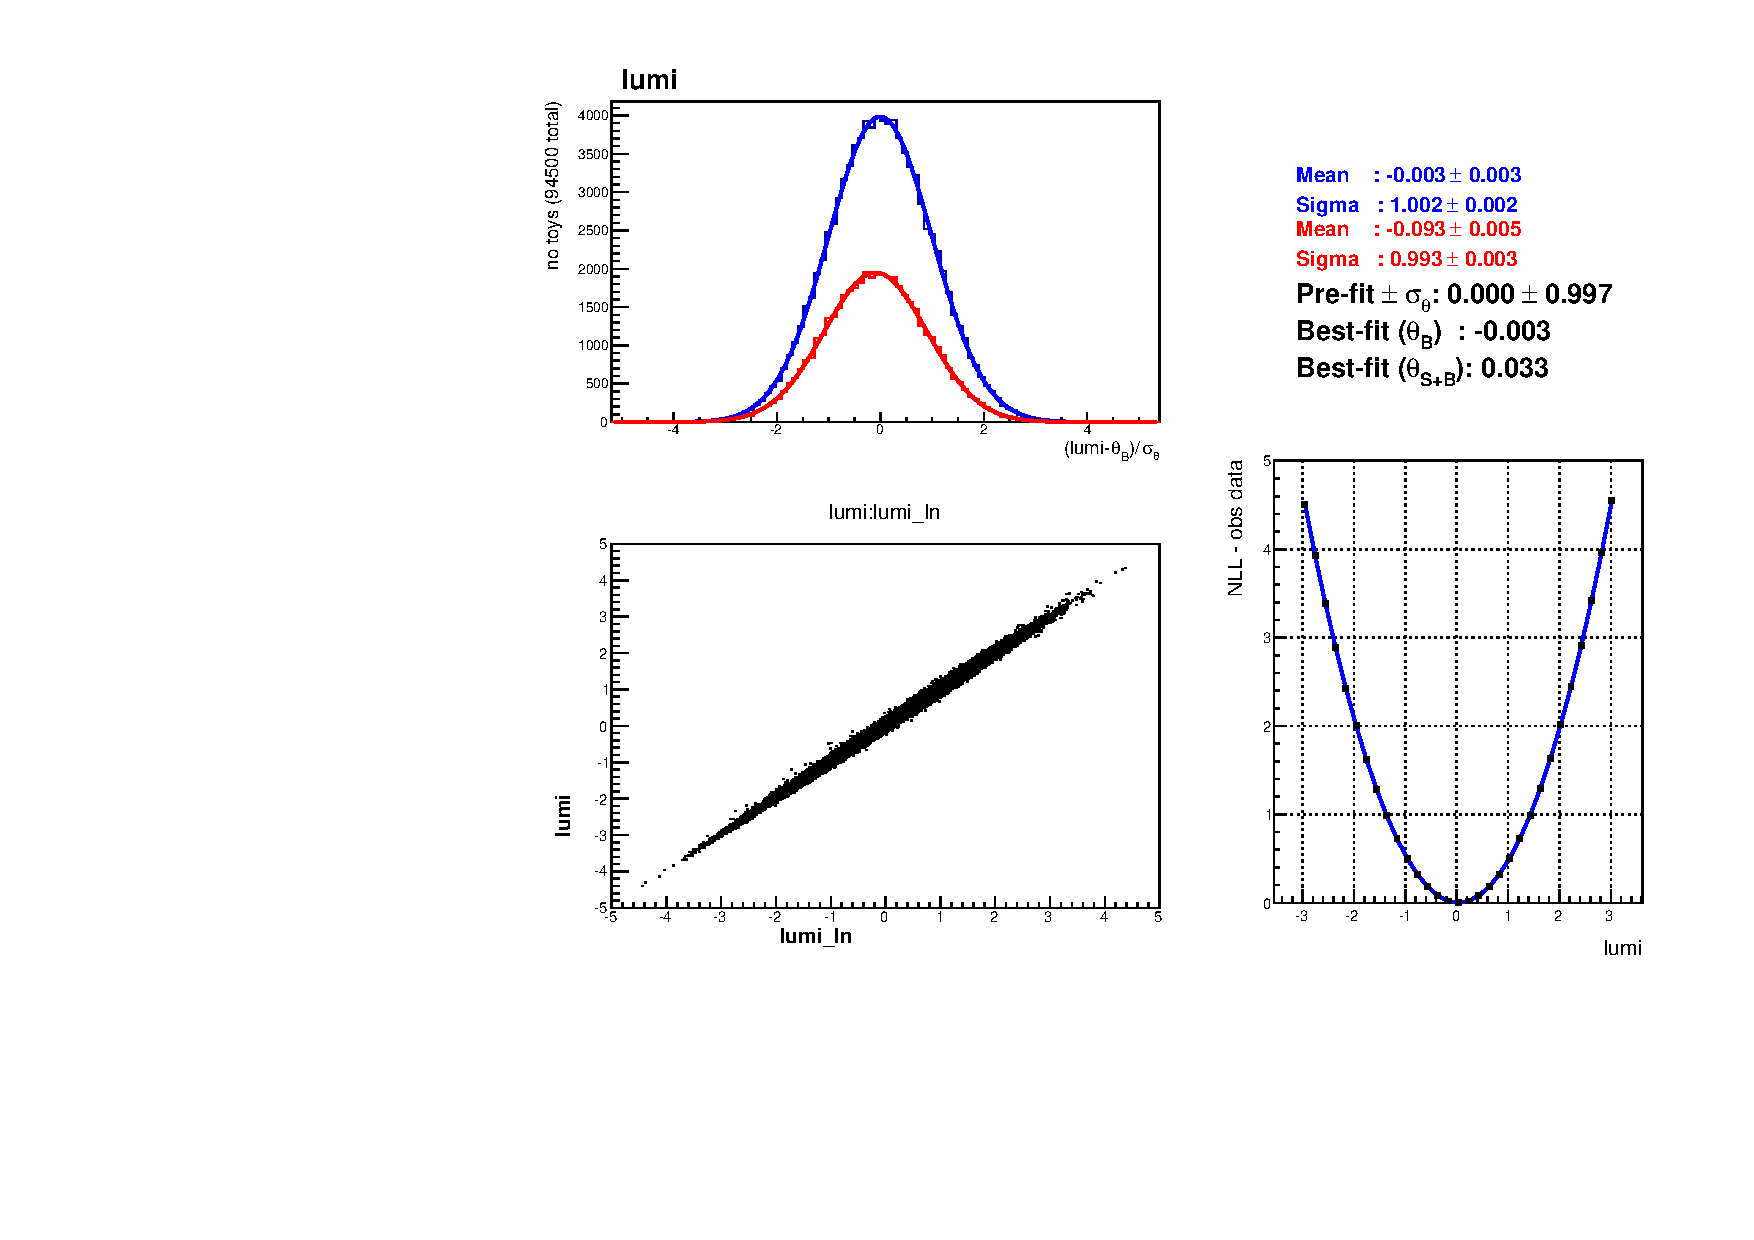
\includegraphics[width=\textwidth]{combinations/diagnostics/tree_fit_sb_lumi.pdf}
    \caption{Summary plots for the parameter \texttt{lumi} of the realistic counting experiment. 
	The entries in the histograms are for fits to toys generated under the background-only
	hypothesis letting $\mu$ float freely. The bottom, left panel shows the correlation
	between the value generated for the pseudo-measurement of the nuisance 
	\texttt{lumi\_In} and the fitted value of the parameter. 
	The lower right panel shows the shape of the 
	negative log-likelihood (NLL) as a function of the nuisance parameter.
	The parameters of the fitted Gaussian for each histogram is given as 
	Mean and Sigma. The value and error of the nuisance are given before fitting
	to the data (Pre-fit), followed by the best fit value of the parameter 
	under the background-only and signal plus background hypotheses.}
    \label{fig:real_lumi_s}
  \end{center}
\end{figure}

\subsection{Higgs Search Combination}
\label{combinedsearchresults}

A search for the SM Higgs boson was performed by combining data recorded at CMS 
at a centre of mass energy of 7 and 8 TeV. The search was performed in five
decay modes, $\Hgg$, $\Hzz$, $\Hww$, $\Htt$ and $\Hbb$ with datasets of
integrated luminosities of $4.9-5.1~fb^{-1}$ and $5.1-5.3~fb^{-1}$
from the 2011 and 2012 data taking periods of the LHC respectively.
The search is performed across a wide range in Higgs mass hypothesis ($\mh$) 
from 110 to 600 GeV. For $\mh>150$, the $\Hgg,~\Htt$ and $\Hbb$ decay modes are nor used
as their expected sensitivities are no longer sensitive compared to the $\Hww$ and
$\Hzz$ channels. Figure~\ref{fig:expectedlimits} shows the relative sensitivities of 
each decay channel in terms of the expected exclusion limit for the size of the dataset 
used. The exclusive final state topologies in each of the five modes used
in the combination, including the size of the dataset used and the mass range to
which they are sensitive, are given in Table~\ref{tab:channelsummary}.

\begin{figure}
\begin{center}
	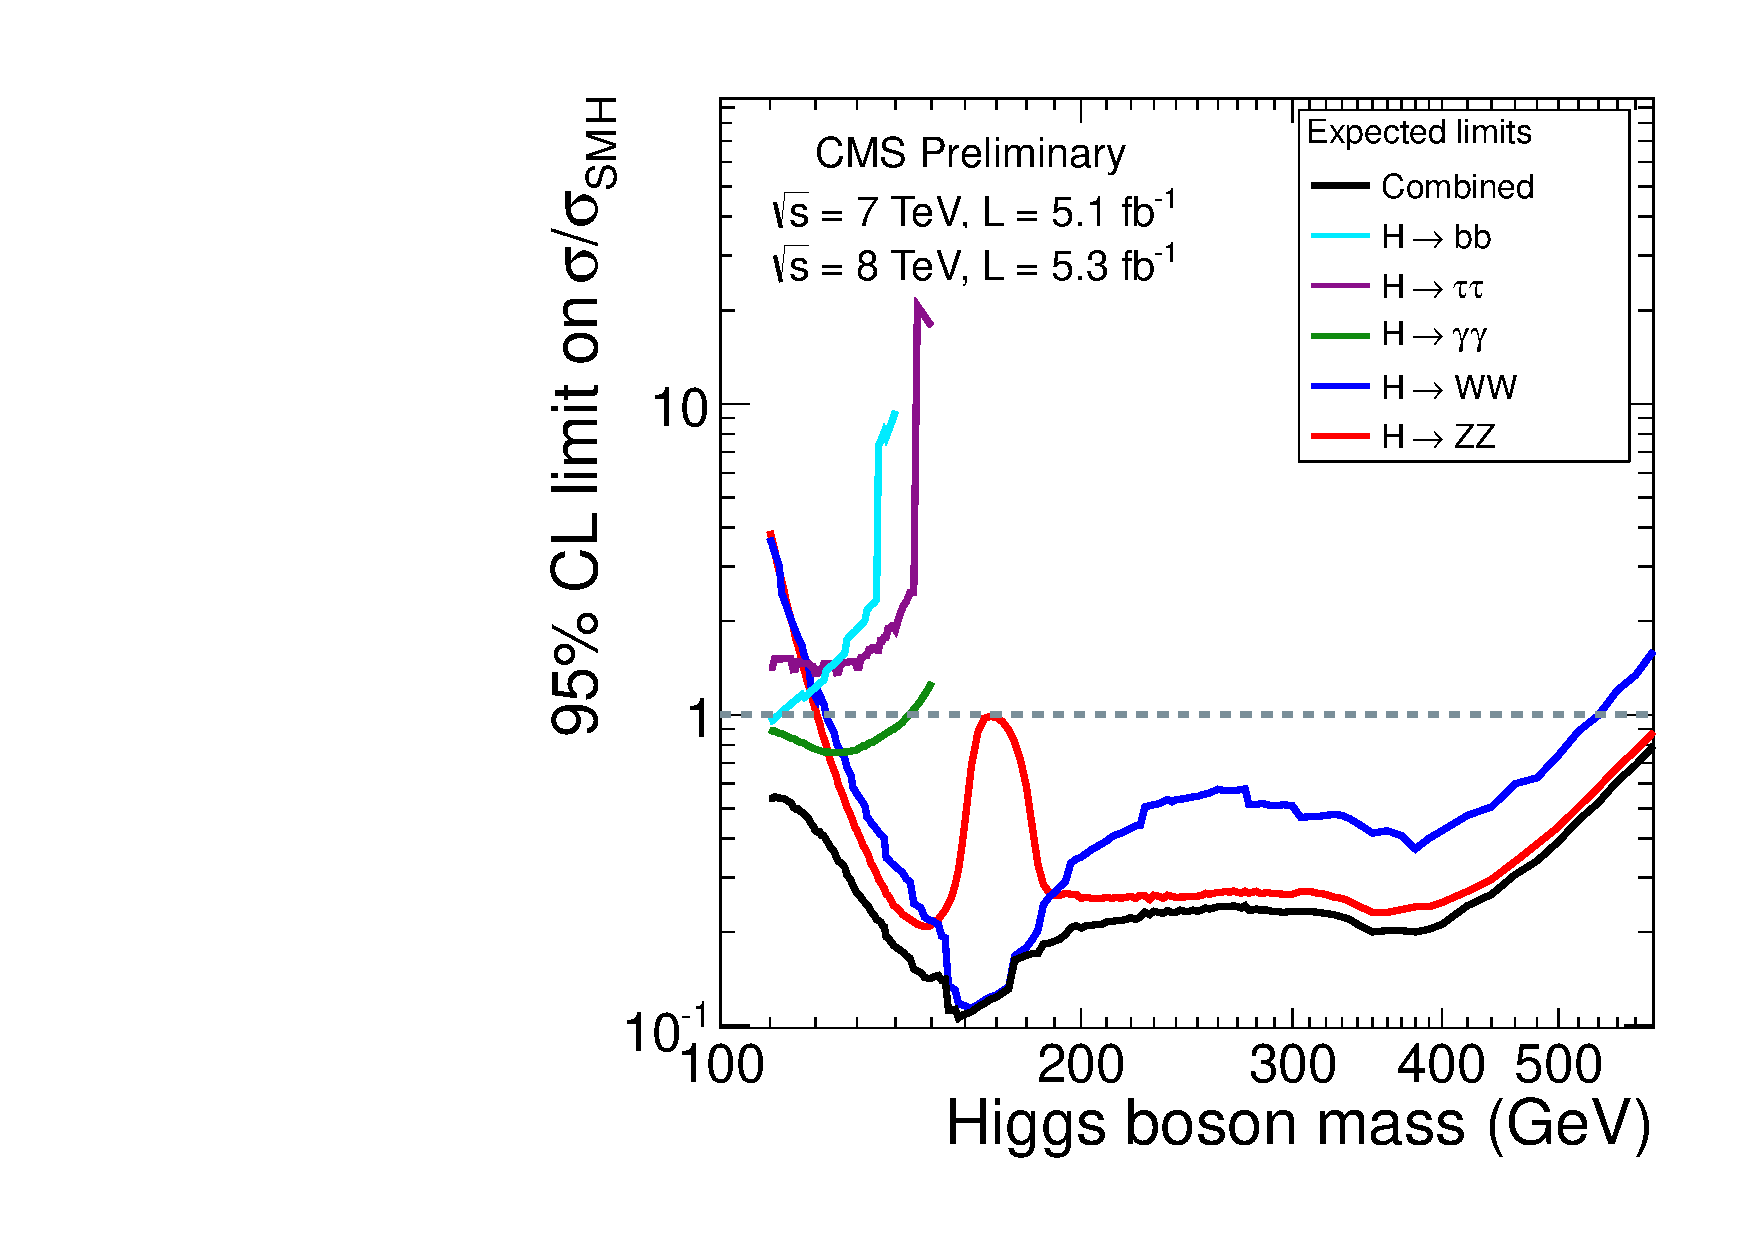
\includegraphics[width=0.49\textwidth]{combinations/ichep2012/Figure_001-a.pdf}
	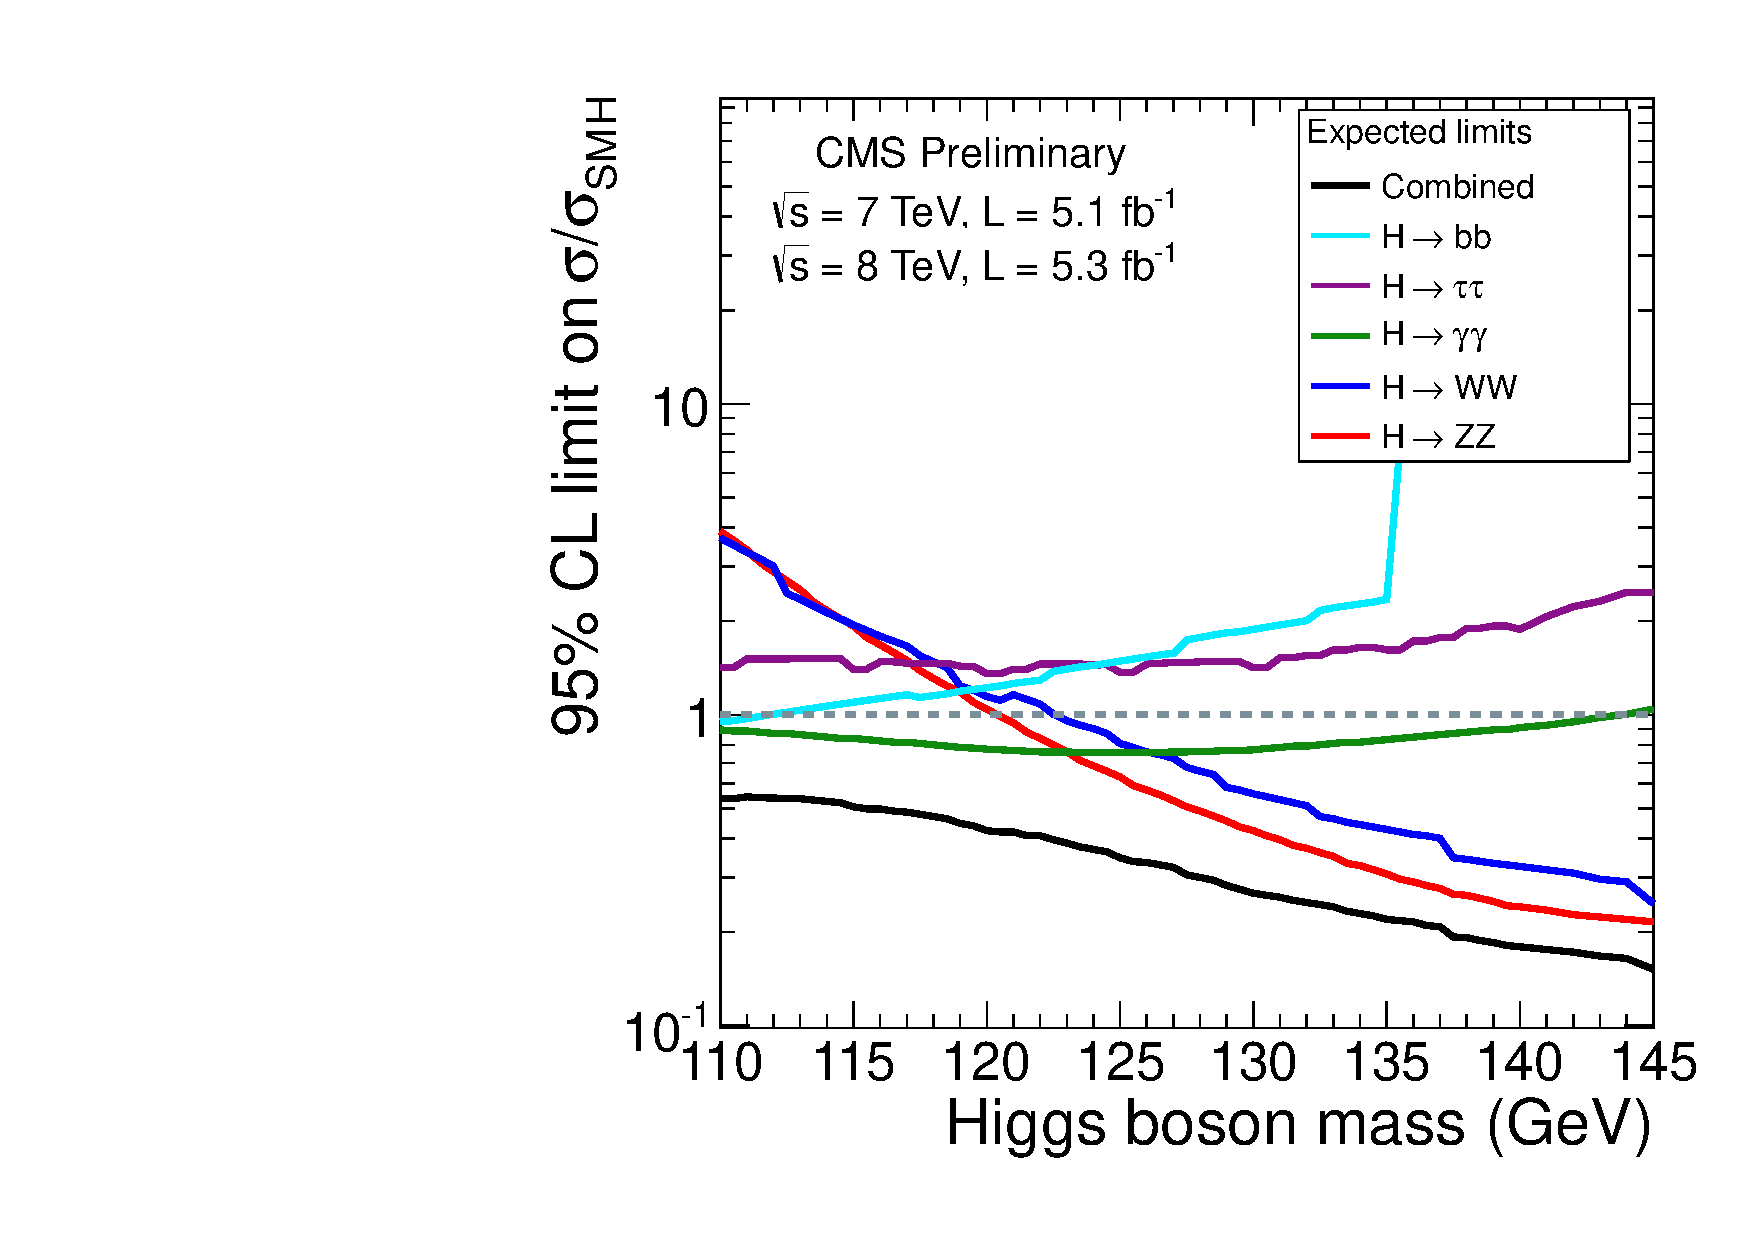
\includegraphics[width=0.49\textwidth]{combinations/ichep2012/Figure_001-b.pdf}
	\caption{Median expected 95\% CL upper limits on $\mu=\xs$ 
	for the five Higgs boson decay channels and their combination in the absence
	of a Higgs boson as a function of $\mh$. The limits are given in the range 
	110-600 GeV (left) and 110-145 GeV (right). A channel which falls below 1,
	indicated by the dashed line, for some range is expected to exclude a Higgs 
	in that range at the 95\% CL using this dataset.}
	\label{fig:expectedlimits}
\end{center}
\end{figure}

\subsubsection{Combined Search Channels}
The $\Hgg$ analysis is one of the most sensitive channels at low $\mh$. The 
analysis is that described in Chapter~\ref{chap:hgg} with the exception of
the signal extraction method. Events are categorized using the diphoton BDT into 
four classes chosen so as to optimise the search in terms of the expected limit
at $\mh=125~GeV$. The diphoton invariant mass spectrum in each category is fit 
with polynomial functions whose order is determined following a procedure designed
to reduce any potential bias to less than 20\% of the statistical uncertainty on 
the background~\citep{HIG-12-015}. The dijet selected events are 
categorised separately and treated in the same way as the inclusive events.

Due to the extremely high cross-section of $b\bar{b}$ production in 
p-p collisions, the $\Hbb$ search focuses on Higgs boson production in association
with a $W$ or $Z$, which are identified by the presence of leptons. In the case 
of neutrino final states such as $Z\rightarrow \nu\nu$, the missing transverse energy 
($\met$) of the event is required to be large indicating momentum propagated out of the detector by the neutrinos~\citep{HIG-12-019}. 
This quantity is defined as the magnitude of the negative vector sum over all energy deposits, 
$E_{k}$, in the calorimeters projected into the transverse plane 
 ($\hat{\mathbf{i}},\hat{\mathbf{j}}$),
\begin{equation}
\met = |\metvec| =|\sum_{deposits} -\sin\theta_{k}\left(E_{k}\cos(\phi_{k})\hat{\mathbf{i}}+E_{k}\sin(\phi_{k})\hat{\mathbf{j}}\right)|
\end{equation}
The Higgs candidate itself is reconstructed by looking for two 
$b$-tagged jets indicated by their production at secondary vertices. Events are 
categorized into those where the 
$W$ or $Z$ boson is recoiling away from the $b\bar{b}$ system with high momentum.
The main backgrounds are from $W/Z$+jets and $t\bar{t}$ as well as from $WZ$ and $ZZ$
in which the $Z$ decays to a pair of $b$-quarks. The backgrounds are suppressed
by use of a multivariate analysis technique trained on MC simulation.
The search is also performed in events in which the Higgs is produced in association
with a pair of top-quarks ($ttH$) categorized into either lepton plus jet or dilepton 
final states~\citep{HIG-12-019}. This mode was not included in the 8 TeV dataset
for the ICHEP 2012 combination.

In the $\Htt$ decay channel, the search is performed using events with leptonic
final states and events in which one of the tau-leptons decays hadronically 
($\tau_{h}$)~\citep{HIG-12-018}.
Events are divided into categories based on the number and type of jets in the event
and by the transverse momentum of the visible part of the tau decay.
A signal in this channel will be visible as a broad excess in the invariant mass
of the $\tau\bar{\tau}$ system ($m_{\tau\tau}$). The main backgrounds are from
$Z\rightarrow\tau\tau$ events and $W+$jet production. 
Production of $qqH$ is tagged by the association of two jets consistent with 
those resulting from vector boson fusion. Finally, the $VH$ modes are
exploited by selecting events which have one or more additional leptons 
consistent with a $W$ or $Z$ boson decay.

The $\Hww$ analysis is one of the most sensitive analyses at CMS for
values of $\mh$ between 150 and 200 GeV~\citep{HIG-12-017}. 
The $WW\rightarrow2l2\nu$ sub-channel consists of events with 
two oppositely charged leptons, a large $\met$ and up 
to two jets (to target $qqH$ production).
These are sub-divided into categories in which the two leptons
are of the same or opposite flavour to exploit the different
background contributions from $Z$ decays. For the 7TeV analysis,
an MVA classifier was trained on signal and background 
MC to separate signal from background. The search is conducted by looking 
for an excess of events in the output distribution of the MVA.
In the $WW\rightarrow l\nu 2q$ sub-channel, a broad excess is searched
for in the four-body invariant mass~\citep{HIG-12-021}. 
The invariant mass is reconstructed from the lepton four-vector and $\metvec$ 
assuming the mass of the $l\nu$ is that of a $W$ boson and 
choosing the neutrino's longitudinal component to be that which minimises 
the transverse momentum of the $l\nu$ system.
Associated production of the Higgs with a $W$ boson is searched for 
by looking for an excess of events with three leptons and large 
$\met$~\citep{HIG-11-034}.

The $\Hzz$ analysis focuses on four final state topologies.
The $ZZ\rightarrow 4l$ is a search for a narrow four-lepton invariant mass 
peak over a small background~\citep{HIG-12-016}. The kinematics of the $4l$ system are used
to assign a probability that the event is from either a signal or background 
process to improve the sensitivity. For the lower mass region ($m_{H}<180$ GeV),
only one of the lepton pairs is required to have a mass consistent with an 
on-shell $Z$ boson.
The $4e$, $4\mu$ and $2e2\mu$ sub-channels are categorised separately as the 
mass resolutions and the background rates differ between between the three 
final states. In the $ZZ\rightarrow 2l2\tau$ and $ZZ\rightarrow 2l2q$ channels, 
a broader peak is searched for in the dilepton-ditau and dilepton-dijet
mass respectively~\citep{HIG-12-016,HIG-11-027}. 
The limited resolution in jet energy reconstruction
and the effect of the neutrino escaping detection in leptonic tau decays
degrades the mass resolution in these channels compared to the $4l$ decay.
The $ZZ\rightarrow 2l2\nu$ search looks for a leptonic $Z$ decay
and a large $\met$~\citep{HIG-12-023}.
In this channel, the decay is not fully reconstructible and so a measure of the mass
is given by the transverse mass, $m_{T}$ defined as,
\begin{equation}
m_{T} = \left[2 p_{T}^{Z}\met(1-\cos(\Delta\phi))\right]^{\frac{1}{2}},
\end{equation}
where $p_{T}^{Z}$ is the transverse momentum of the dilepton system and 
$\Delta\phi$ is the angle in the transverse plain between that momentum vector and 
$\metvec$.
A broad excess of events in the $m_{T}$ distribution is used to signal the presence 
of a SM Higgs boson.


\begin{sidewaystable}
\centering
\begin{tabular}{|l|c|l|c|c|c|}
\hline
\textbf{$H$ decay} & \textbf{$H$ prod} & \textbf{Final state} 
& \textbf{No. sub-chans} & \textbf{$\mh$ (GeV)}
& \textbf{Lumi $(fb^{-1})$ 7/8TeV} \\
\hline
\hline
$\gamma\gamma$ 	 & untagged & $\gamma\gamma$ (kinematic classes) & 4 & 110-150 & $5.1/5.3$ \\
	& $qqH$-tag & $\gamma\gamma+jj$ ($m_{jj}$ classes in 8TeV) & 1 or 2  & 110-150 & $5.1/5.3$ \\
\hline
$bb$  & $VH$-tag & $(\nu\nu,ee,\mu\mu,e\nu,\mu\nu + 2 j_{b})\times$(low/high~$p_{T}^{V}$)
 & 10 & 110-135 & $5.0/5.1$ \\

 & $ttH$-tag & $l+(4,5,\ge6 j)\times~(3,\ge4 j_{b}),~l+4j +2j_{b}$,& 9 & 110-140 & $5.0/-$  \\
 &  	     &  $ll+(2,\ge3 j_{b})$ 				   & &   &  \\
\hline

$\tau\tau$ & $0/1-\textrm{jets}$ & $(e\tau_{h},\mu\tau_{h},e\mu,\mu\mu)\times
			(\textrm{low/high}~p_{T}^{\tau\tau})\times(0/1j)$ 
	& 16 & 110-145 & $4.9/5.1$ \\
 & $qqH$-tag & $ (e\tau_{h},\mu\tau_{h},e\mu,\mu\mu) + jj$ 
	& 4 & 110-145 & $4.9/5.1$ \\
 & $ZH$-tag & $ (ee,\mu\mu)\times(\tau_{h}\tau_{h},\mu\tau_{h},\mu\tau_{h},e\mu)$ 
	& 8 & 110-160 & $5.0/-$ \\
 & $WH$-tag & $ ee\tau_{h},\mu\mu\tau_{h},e\mu\tau_{h}$ 
	& 3 & 110-140 & $4.9/-$ \\
\hline
$WW\rightarrow l\nu l\nu$ & $0/1-\textrm{jets}$ & $(ee/\mu\mu,e\mu)\times(0/1j)$ 
	& 4 & 110-600 & $4.9/5.1$ \\
$ $ & $qqH$-tag & $(l\nu l\nu + jj)$ (SF or OF $ll$ in 8TeV)  
	& 1 or 2 & 110-600 & $4.9/5.1$ \\
$ $ & $WH$-tag & $3l 3\nu$ 
	& 1 & 110-200 & $4.9/-$ \\
$ $ & $VH$-tag &$(l\nu l\nu + jj)$ (SF or OF $ll$) 
	& 2 & 118-190 & $4.9/-$ \\
$WW\rightarrow l\nu qq$ & untagged & $(e\mu)\times(jj+0/1j)$ 
	& 4 & 170-600 & $5.0/5.1$ \\
\hline
$ZZ\rightarrow 4l$ & untagged  & $4e,4\mu,2e2\mu$ & 3 & 110-600 & $5.0/5.3$ \\
$ZZ\rightarrow 2l2\tau$ & untagged  
	& $(ee,\mu\mu)\times(\tau_{h}\tau_{h},e\tau_{h},\mu,\tau_{h} ,e\mu)$ 
	& 8 & 200-600 & $5.0/5.3$ \\
$ZZ\rightarrow 2l2q$ & untagged  
	& $(ee,\mu\mu)+jj (0,1,2 j_{b})$  
	& 6 & 200-600 & $4.9/-$ \\
$ZZ\rightarrow 2l2\nu$ & untagged  
	& $(ee,\mu\mu)+\slash{E_{T}} (0,1,2 j)$ (not $qqH$ jets)  
	& 6 & 200-600 & $4.9/5.1$ \\
$ $ & $qqH$-tag 
	& $(ee,\mu\mu)+\slash{E_{T}} + jj $   
	& 2 & 200-600 & $4.9/5.1$ \\
\hline
\end{tabular}
\caption{Summary of analyses included in the ICHEP 2012 combination~\citep{HIG-12-020}. 
The column for $H$ prod indicates the production process targeted by the sub-channel.
A label ``untagged'' indicates that the main contribution is from the $ggH$ production process.
The final states for each channel are exclusive (no events lie in more than one sub-channel.
The notations used here are: $jj$ indicating a dijet pair whether from a $W,Z$ decay or 
being consistent the vector-boson fusion process; $j_{b}$ denotes a jet which is 
identified as a $b$-jet; 
$l$ is either a muon ($\mu$) or electron ($e$); OF and SF are dilepton pairs with 
opposite flavour ($e\mu$) and same flavour ($ee$ or $\mu\mu$) respectively.}
\label{tab:channelsummary}
\end{sidewaystable}

\subsubsection{Combined Results}
\label{sec:combinedsearchresults}
The 95\% upper limits on the signal strength $\mu=\xs$ as a function 
of the hypothesised Higgs boson mass, $\mh$, are shown in 
Figure~\ref{fig:combinedexcl}. The right hand figure is an enlargement of
the region $110 < \mh  < 145 GeV$. The median expected limit in the absence
of a SM Higgs boson is less than 1 for the range $110< \mh<600 GeV$. 
The observed limits are consistent with statistical fluctuations given the 
size of the dataset in most of the range as indicated by the fact that the 
observed line lies within the 68\% or 95\% quantiles. However an
excess of events is observed at low mass in the range $122.5  < \mh < 127 GeV$
so that exclusion of a SM Higgs boson with a mass in that range cannot be excluded
at the 95\% confidence level. The significance of the excess is quantified as a function
of $\mh$ by calculating the local $p$-value, $p_{0}$ as shown in Figure~\ref{fig:combinedpval}. 
For the overall combination, the local $p_{0}$ is around $5.5\times10^{-7}$, 
equivalent to a significance of $4.9\sigma$. The test indicates that the observed excess 
is incompatible with the background-only hypothesis indicating the presence of 
a new state with a mass near 125 GeV.
The largest contributions to the excess are
from the $\Hgg$ and $H\rightarrow ZZ\rightarrow4l$ channels, 
both of which have good mass resolutions and hence a good localisation
of the excess. The combination of the two 
high mass resolution channels results in a local significance of $5\sigma$. 
Of the lower resolution channels, only $\Hww$ shows an excess at 125 GeV. The inclusion
of the $\Hbb$ and $\Htt$ channels reduced the overall significance.
The overall global $p$-value in the range 115-130 GeV is calculated by 
generating 10,000 pseudo-datasets and fitting for the constant $C$ in 
the relationship to the local $p$-value given in Equation~\ref{eqn:lee} 
(see Figure~\ref{fig:leecombination}). The
look-elsewhere effect, calculated as the ratio between the local and global $p_{0}$, 
is around 11 such that the global significance remains high at $4.4\sigma$.

\begin{figure}
\begin{center}
 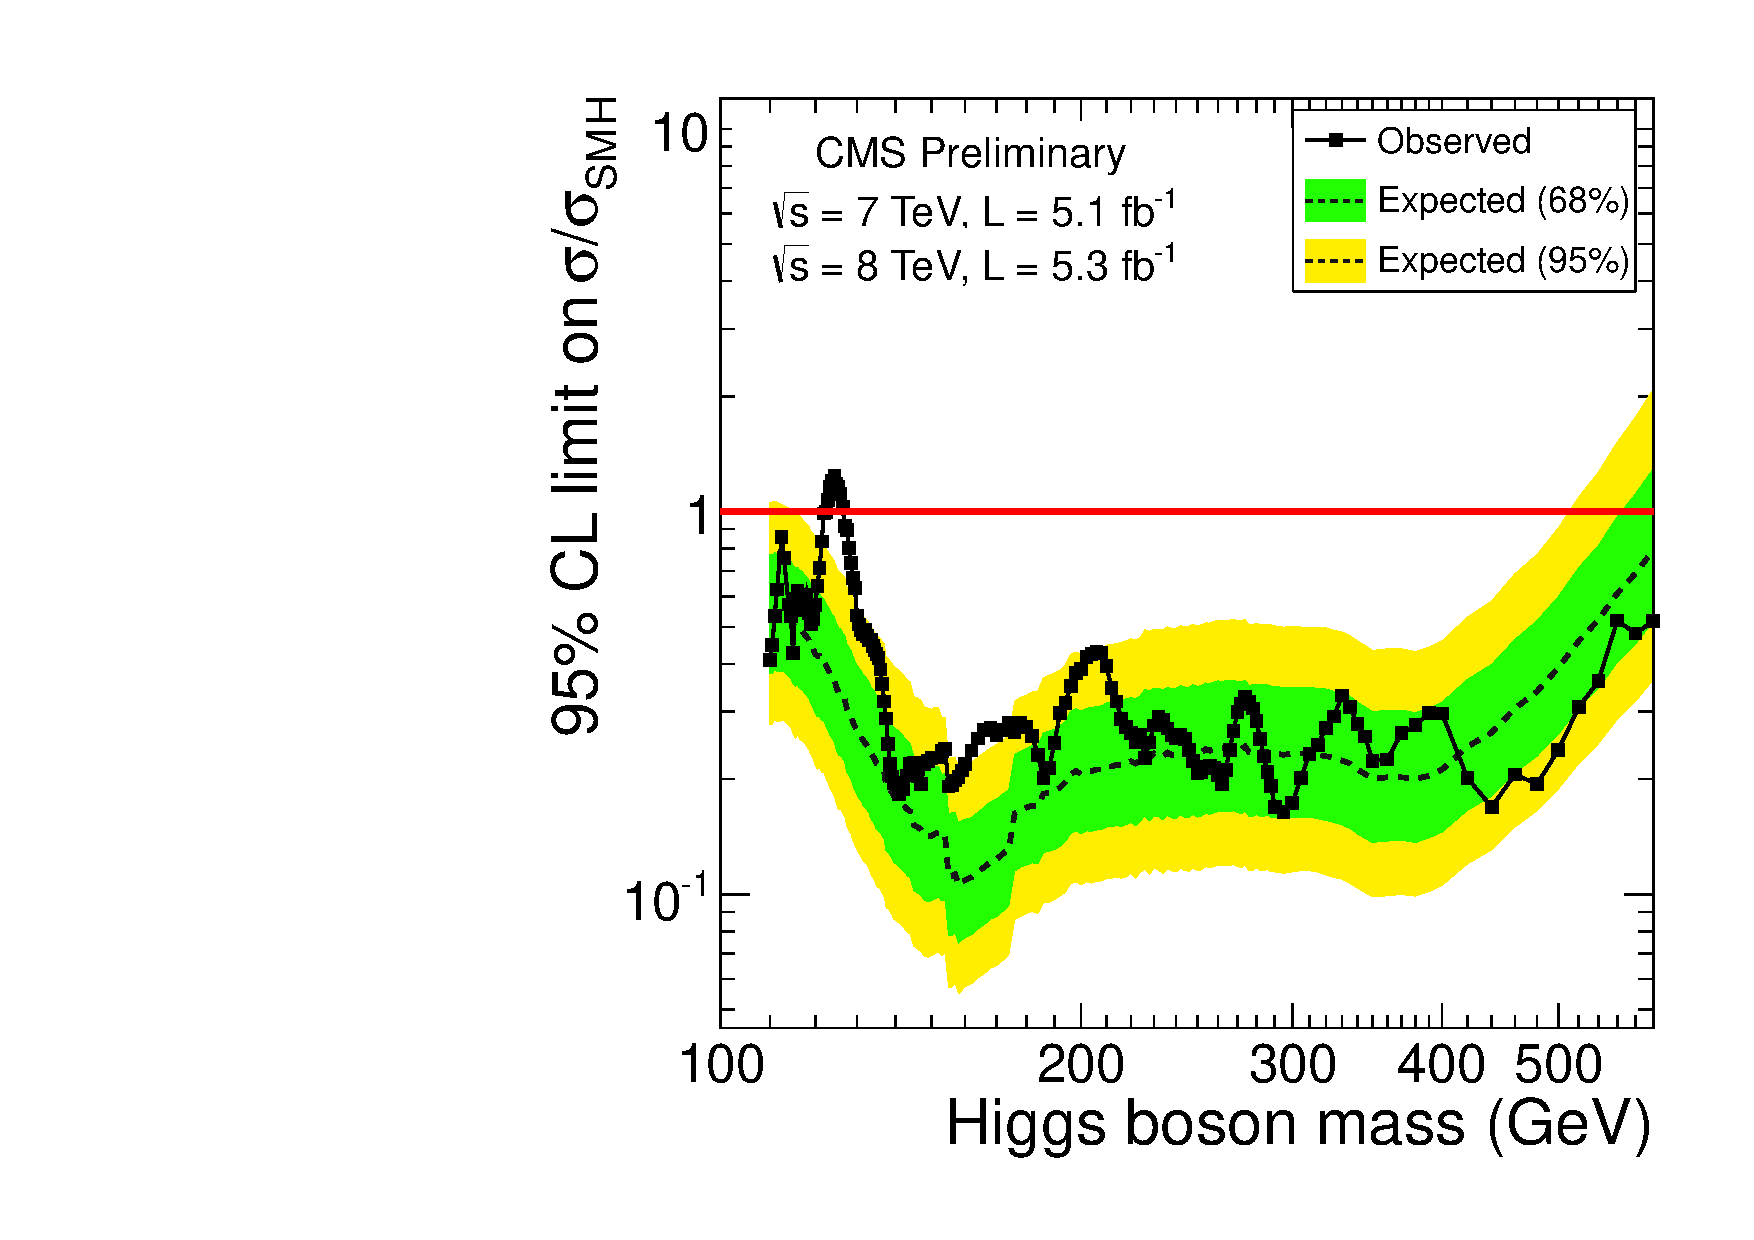
\includegraphics[width=.49\textwidth]{combinations/ichep2012/Figure_004-a.pdf}
 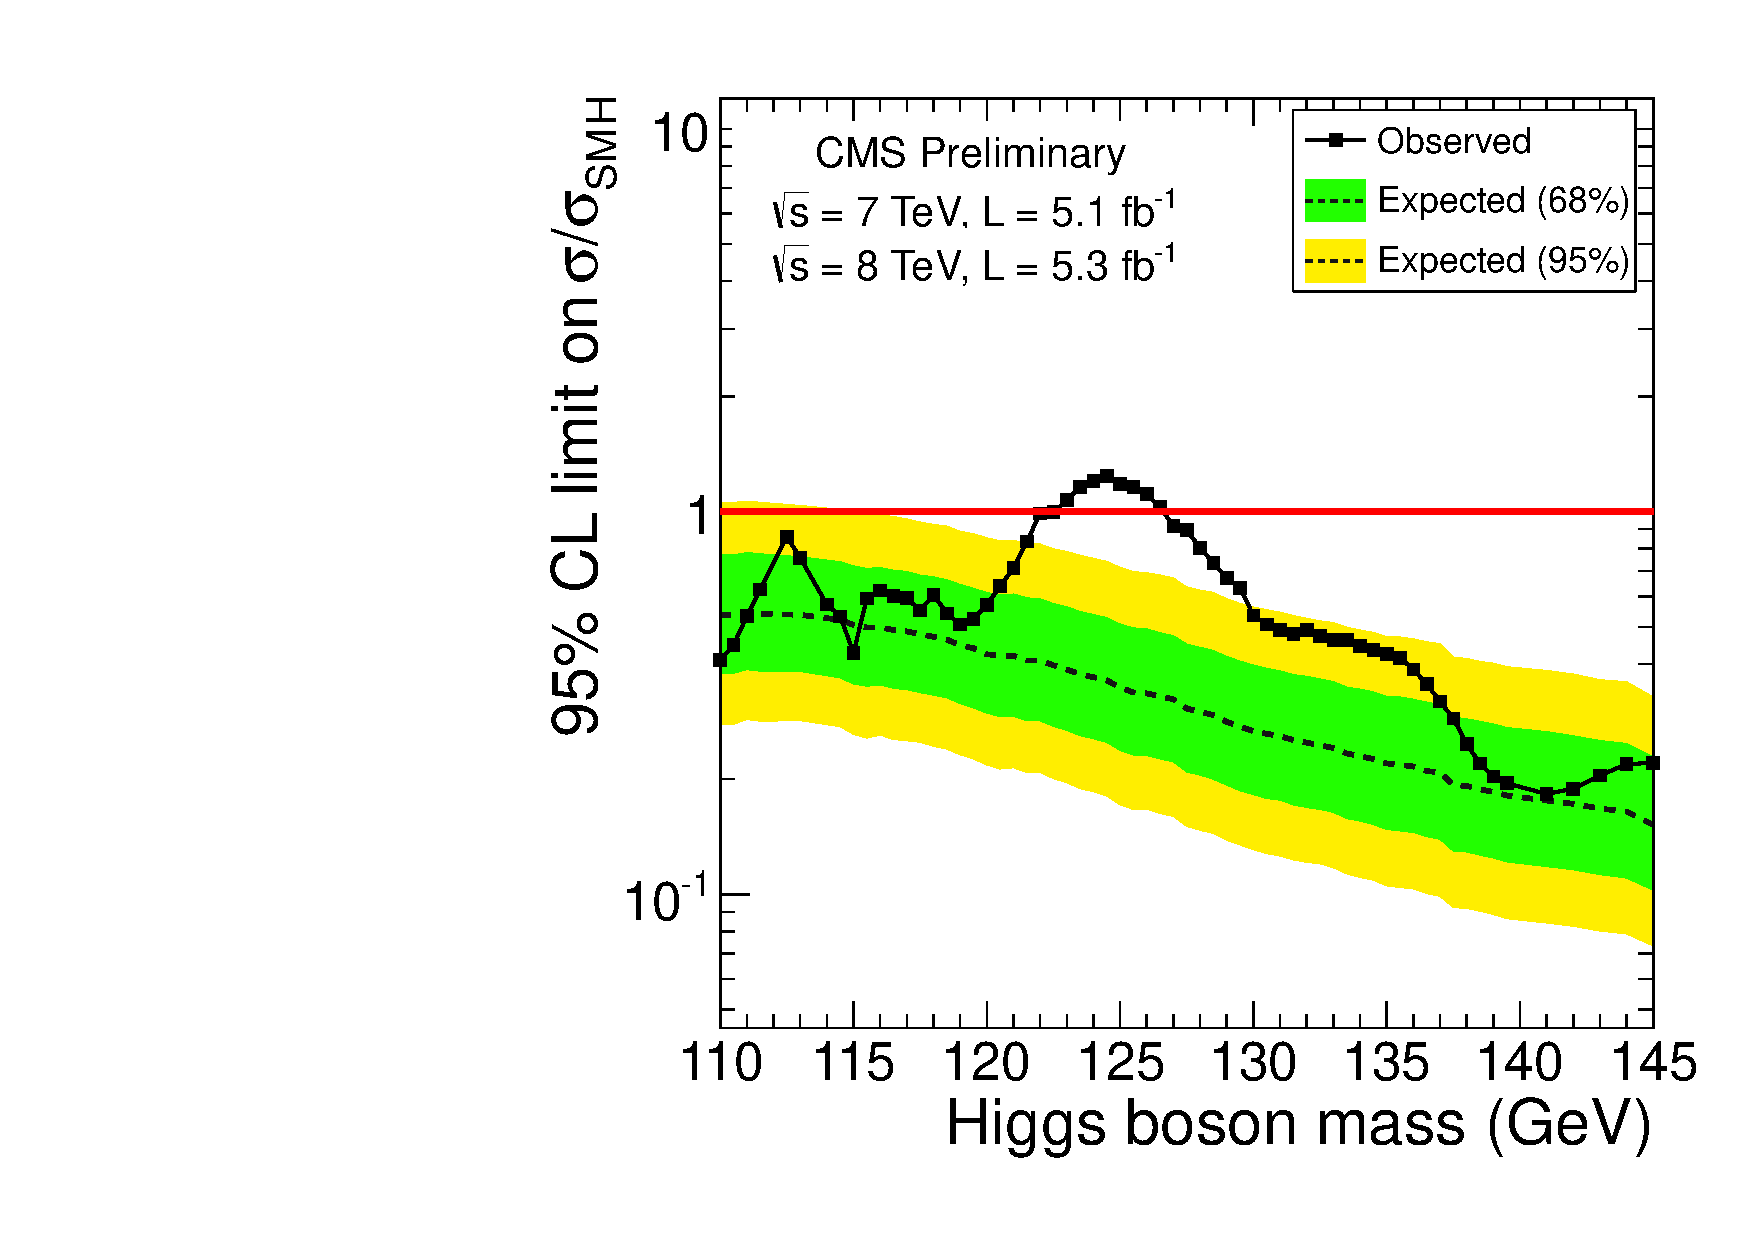
\includegraphics[width=.49\textwidth]{combinations/ichep2012/Figure_004-b.pdf}
 \caption{Combined 95\% upper limits on the production cross-section of Higgs boson
production relative to that of the Standard Model in the $\mh$ ranges 110-600 GeV (left)
and 110-145 GeV (right). The median upper limits expected in the absence of a SM Higgs
are indicated by the dashed black line and the 68\% and 95\% quantiles by the green and yellow
bands respectively.
The observed upper limits from the combined ICHEP 2012 dataset is shown by the black solid line.
Where the observed limit is lower than 1 (red line), a SM Higgs boson with that $\mh$ 
is excluded at the 95\% confidence level.}
\label{fig:combinedexcl}
\end{center}
\end{figure}

\begin{figure}
\begin{center}
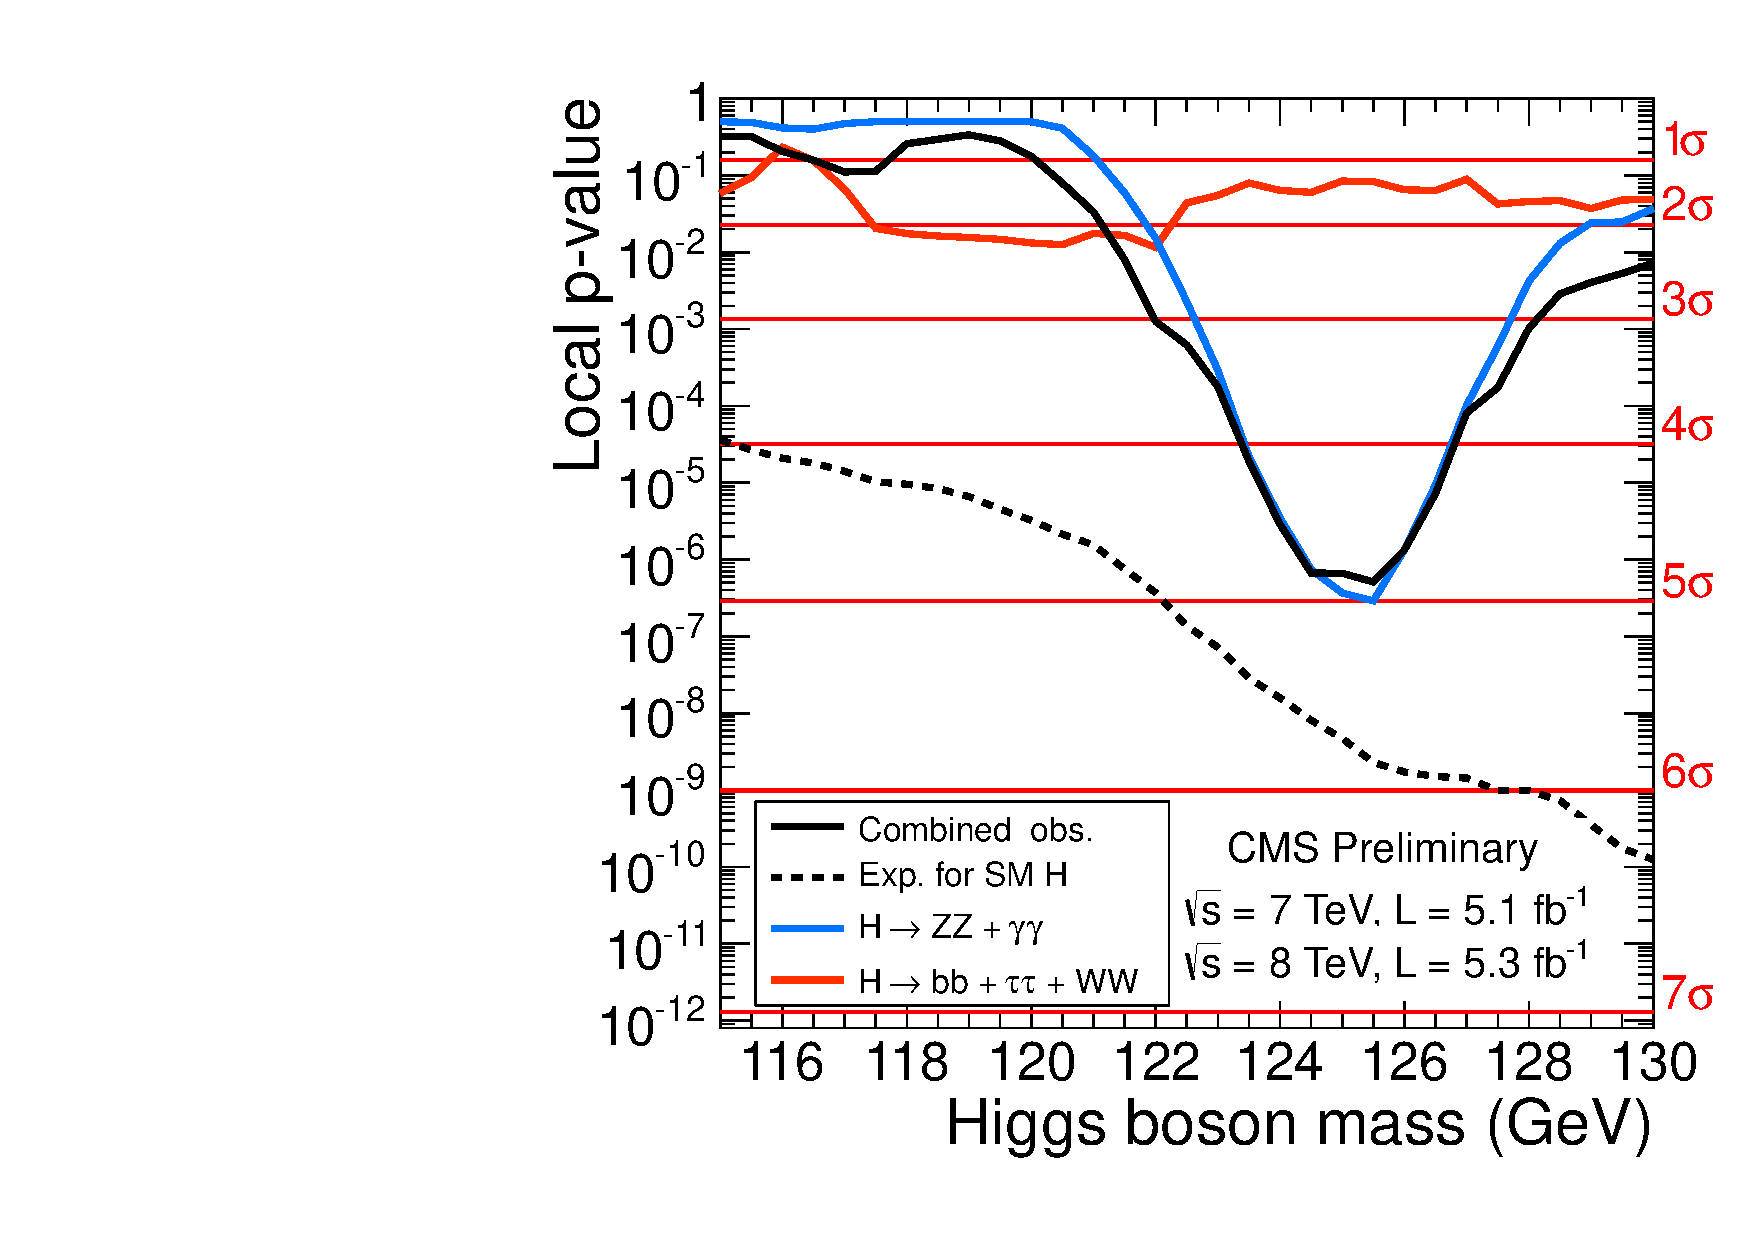
\includegraphics[width=.8\textwidth]{combinations/ichep2012/sqr_pvala_all_byresol.pdf}
\caption{The observed local $p$-value, $p_{0}$ for sub-combinations of the low and
high resolution channels and the overall combination as a function of $\mh$. The dashed
line shows the expected $p_{0}$ at each $\mh$ should a SM Higgs boson exist with mass $\mh$.}
\label{fig:combinedpval}
\end{center}
\end{figure}


\begin{figure}
\begin{center}
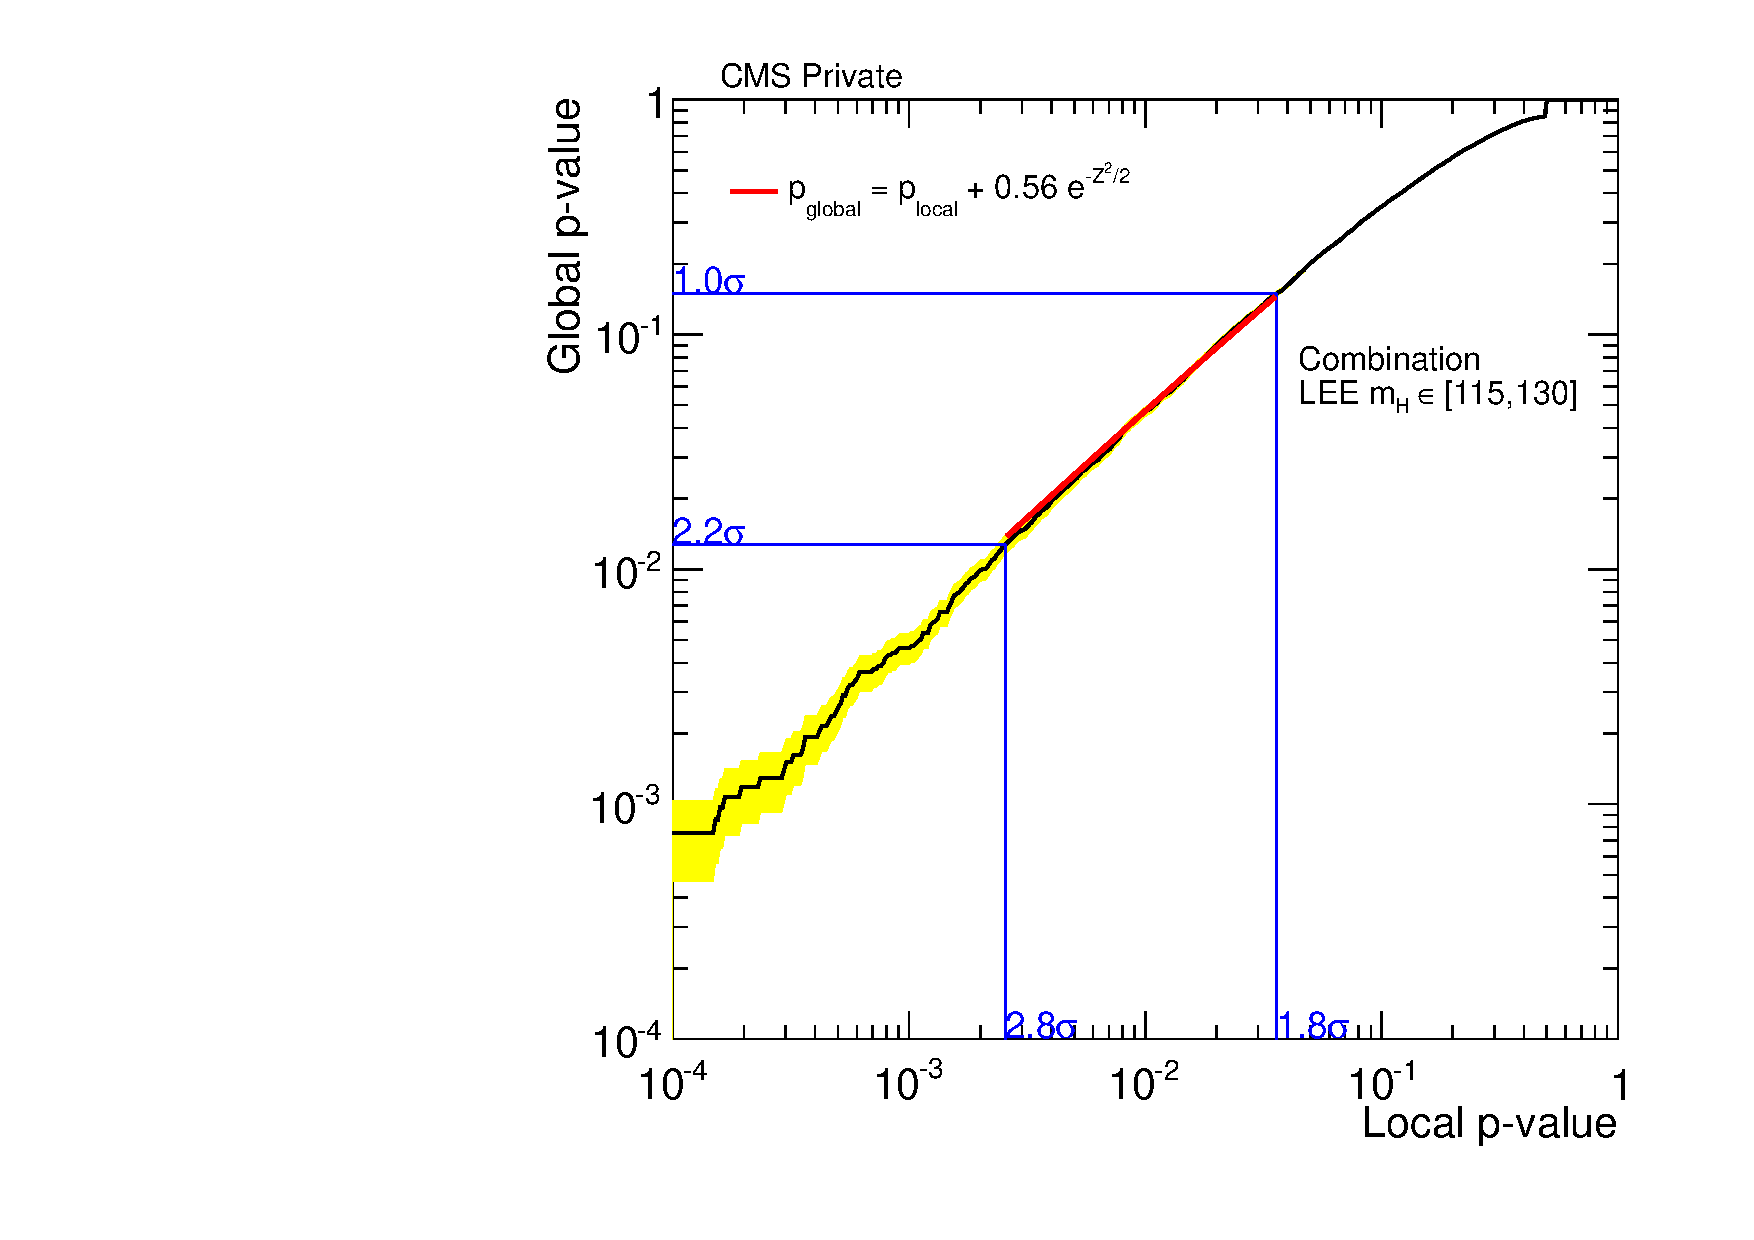
\includegraphics[width=.8\textwidth]{combinations/ichep2012/lee-combination-115-130.pdf}
\caption{Relationship between the local and global $p_{0}$ in the range 115-130 GeV.
The red line indicates the analytic expression (shown) which is fit to the relationship derived from
10,000 pseudo-datasets.}
\label{fig:leecombination}
\end{center}
\end{figure}
